%   ------------------------------------------------------------------------
\FloatBarrier
\section{Análise do Animated Drawnings}
\label{s.sketchLab}

A ferramenta Animated Drawnings, encontrada na plataforma AI Demos da Meta\footnote{https://aidemos.meta.com/}, implementa o algoritmo para animação de desenhos proposto por \cite{animated10.1145/3592788}. A tecnologia, conforme descrita no artigo, visa animar automaticamente desenhos infantis de figuras humanoides, contendo diversas opções específicas de animações com movimentos e poses definidas. A IA é completamente gratuita, porém seu termo não permite o uso comercial das animações geradas (Figura \ref{fig:sketchInicial} no Apêndice \ref{ap.telasIA}). Seu foco em desenhos amadores facilita o reconhecimento de personagens com traços mais simples e abstratos.

Para os testes, o objetivo era produzir uma animação do personagem andando a partir do sprite dele. Como o algoritmo exige que os membros do personagem não estejam sobrepostos (Figura \ref{fig:sketchSobreposicao} no Apêndice \ref{ap.telasIA}), foi selecionado o sprite de Luz para submissão.

\begin{figure}[htbp]
    \centering
    \caption{\small Sprites usados para o teste no Animated Drawnings}
    \label{fig:sketchArtefatos}
    \begin{subfigure}{0.32\linewidth}
        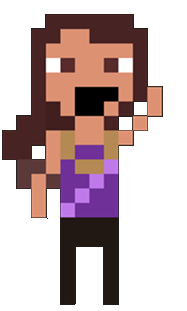
\includegraphics[width=1\linewidth]{figs/sprites/irma.PNG}
        \caption{\small Sprite original da personagem Luz}
        \label{fig:sketchIrma1}
    \end{subfigure}
    \begin{subfigure}{0.32\linewidth}
        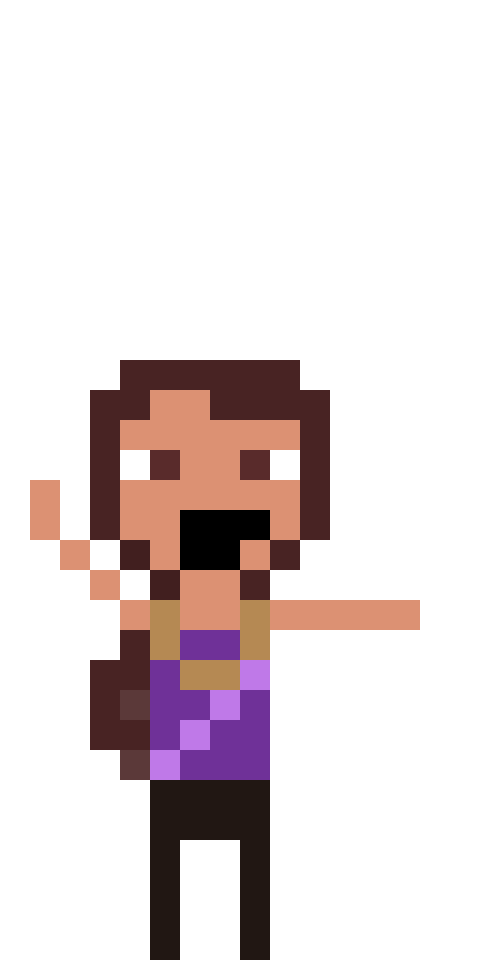
\includegraphics[width=1\linewidth]{figs/sprites/irma_bracos_abertos.png}
        \caption{\small Sprite da Luz sem o cabelo sobrepondo o braço}
        \label{fig:sketchIrma2}
    \end{subfigure}
    \begin{subfigure}{0.32\linewidth}
        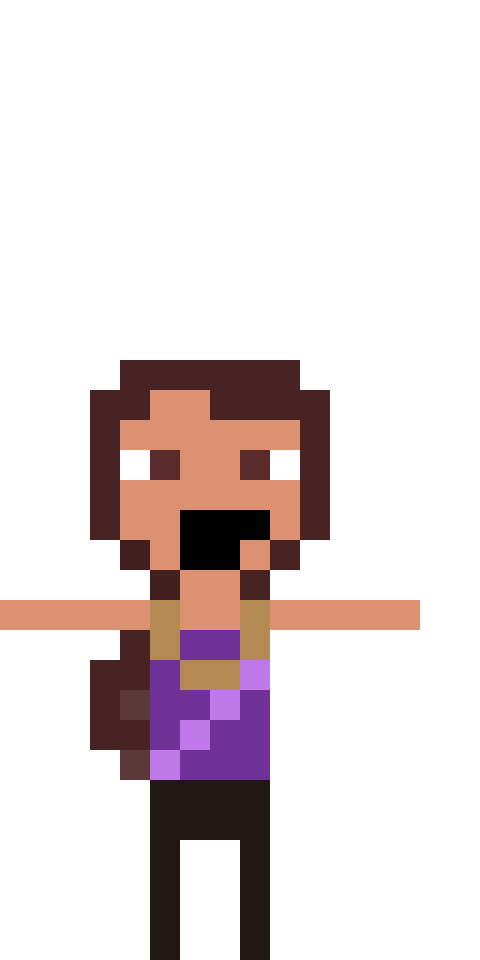
\includegraphics[width=1\linewidth]{figs/sprites/irma_t_pose.png}
        \caption{\small Sprite da Luz com ambos os braços retos}
        \label{fig:sketchIrma3}
    \end{subfigure}

    \legend{\small Fonte: Elaborada pela autora.}
\end{figure}

A geração de qualquer animação requer que o personagem seja primeiramente analisado e reconhecido pela plataforma. Este processo consiste em quatro etapas principais: 

\begin{itemize}
    \item Enviar o desenho, com o personagem a ser animado;
    \item Encontrar o personagem, onde o usuário ajusta a caixa de seleção de maneira que o personagem caiba dentro dela sem sobrar muito espaço;
    \item Destacar o personagem, em que se deve pintar o espaço que o personagem aparece e apagar os lugares que não tem nenhuma parte da pessoa; e
    \item Marcar as articulações do personagem, fase em que se deve posicionar cada bolinha (que representam uma articulação entre: olho, orelha, centro da cabeça, ombro, cotovelo, pulso, quadril, joelho e calcanhar) no lugar correto. 
\end{itemize}

Durante cada um dos processos posteriores ao envio da imagem, o algoritmo realiza uma detecção automática, permitindo que o usuário realize ajustes, se necessário. Após o reconhecimento, existe uma série de animações específicas que podem ser aplicadas ao personagem sem necessidade de prompts textuais.

Na interação inicial (Figura \ref{fig:sketch1} no Apêndice \ref{ap.telasIA}), a ferramenta se mostrou capaz de reconhecer o personagem sem necessidades de ajustes muito grandes. No entanto, a animação formada\footnote{https://drive.google.com/file/d/16zrzJ4IZsnEMS90w3vYGKTGQjKC5adqx/view?usp=sharing} apresentou algumas distorções visíveis(Figura \ref{fig:sketchIrma1Frame}), principalmente no rosto e no cabelo, que se alongavam e entortavam de acordo com o movimento dos braços. Apesar disso, a natureza do algoritmo, que deforma a imagem original em vez de gerar novos quadros do zero, garantiu total consistência com o estilo e design do sprite.O resultado foi avaliado como parcialmente satisfatório: não era um sucesso completo, mas também não era um fracasso.

\begin{figure}[htbp]
    \centering
    \caption{\small Frame da animação gerada pelo Animated Drawnings 1}
    \label{fig:sketchIrma1Frame}
    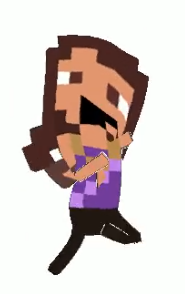
\includegraphics[width=0.3\linewidth]{figs/sketchLab/irma1_frame1_andando.PNG}
    \legend{\small Fonte: Elaborada pela autora, utilizando a ferramenta Animated Drawnings.}
\end{figure}

A análise do resultado indicou que a ferramenta teve dificuldades em separar corretamente as áreas do braço e da cabeça, provavelmente devido à sobreposição do cabelo no desenho original. Para testar essa hipótese, um novo sprite foi desenhado (Figura \ref{fig:sketchIrma2}).

Essa abordagem revelou uma melhora significativa, corrigindo a distorção da cabeça, conforme pode ser vista na comparação de resultados na Figura \ref{fig:sketchCompara1}

%Como a animação tem movimentos específicos pré-determinados, é possível comparar o exato frame específico da pose

\begin{figure}[htbp]
    \centering
    \caption{\small Comparando frames correspondentes}
    \label{fig:sketchCompara1}
    \begin{subfigure}{0.35\linewidth}
        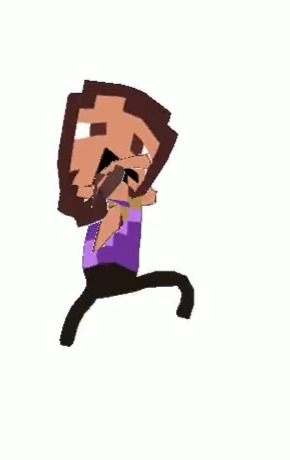
\includegraphics[width=1\linewidth]{figs/sketchLab/irma1_frame2.jpg}
        \caption{\small Frame da animação do sprite original}
        \label{fig:sketchComparaIrma1}
    \end{subfigure}
    \begin{subfigure}{0.35\linewidth}
        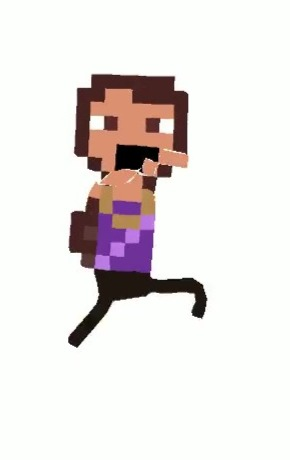
\includegraphics[width=1\linewidth]{figs/sketchLab/irma2_frame2.jpg}
        \caption{\small Frame da animação do sprite modificado}
        \label{fig:sketchComparaIrma2}
    \end{subfigure}

    \legend{\small Fonte: Elaborada pela autora, utilizando a ferramenta Animated Drawnings.}
\end{figure}

Outras animações foram selecionadas para verificar o desempenho da ferramenta em diferentes poses. Os resultados\footnote{https://drive.google.com/drive/u/2/folders/1dFLISEUVXPb-lwEFv5RscT-sCtU-tKsc} se mantiveram consistentes durante todos os testes, como pode ser verificado na Figura \ref{fig:sketchIrma2Frame}. A interação completa pode ser encontrada na Figura \ref{fig:sketch2} do Apêndice \ref{ap.telasIA}.

\begin{figure}[htbp]
    \centering
    \caption{\small Frames das animações geradas pelo Animated Drawnings 2}
    \label{fig:sketchIrma2Frame}
    \begin{subfigure}{0.2\linewidth}
        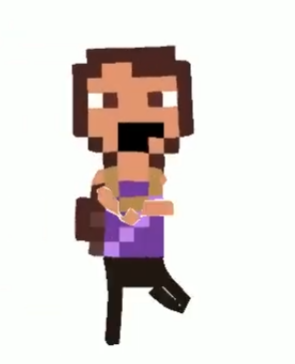
\includegraphics[width=1\linewidth]{figs/sketchLab/irma2_frame1_andando.PNG}
        \caption{\small Frame da animação de andar pulando}
        \label{fig:sketchIrma2Frame1}
    \end{subfigure}
    \begin{subfigure}{0.2\linewidth}
        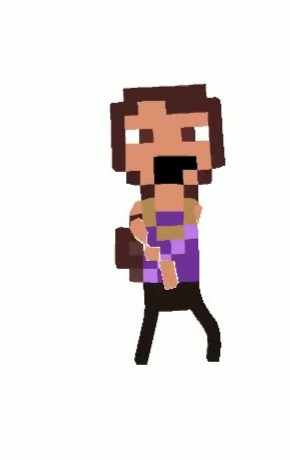
\includegraphics[width=1\linewidth]{figs/sketchLab/irma2_frame1.jpg}
        \caption{\small Frame da animação de andar longe da câmera}
        \label{fig:sketchIrma2Frame2}
    \end{subfigure}
    \begin{subfigure}{0.2\linewidth}
        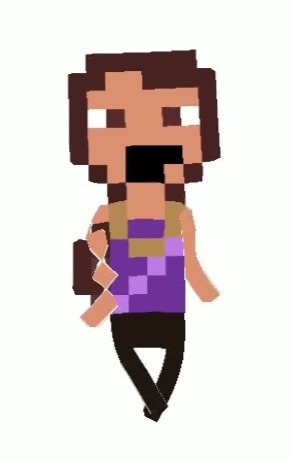
\includegraphics[width=1\linewidth]{figs/sketchLab/irma2_frame3.jpg}
        \caption{\small Frame da animação de andar perto da câmera}
        \label{fig:sketchIrma2Frame3}
    \end{subfigure}
    \begin{subfigure}{0.2\linewidth}
        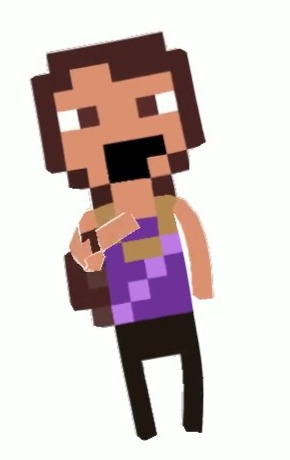
\includegraphics[width=1\linewidth]{figs/sketchLab/irma2_frame4.jpg}
        \caption{\small Frame da animação de acenar}
        \label{fig:sketchIrma2Frame4}
    \end{subfigure}

    \legend{\small Fonte: Elaborada pela autora, utilizando a ferramenta Animated Drawnings.}
\end{figure}

Apesar do sucesso na correção da distorção, um problema fundamental foi observado: as transformações que o sprite sofre fazem com que a animação perca o estilo pixel perfect. Este efeito, já presente no resultado anterior, é uma consequência direta da abordagem da ferramenta, que deforma a imagem em vez de recriá-la quadro a quadro. Não se trata de um erro de implementação, mas de uma incompatibilidade inerente entre a técnica de deformação e a estética específica da pixel art, não ocorrendo em outros estilos 2D.

%Porém, é possível notar que as transformações que o sprite sofre fazem com que a animação perca o estilo de pixel art, apesar do personagem em si ainda manter essa característica. Isso era um problema também no resultado anterior, e dada a natureza da ferramenta (de não gerar uma imagem nova e apenas mover partes da pessoa previamente desenhada), esse defeito vai se manter em qualquer desenho pixelizado. Não é um erro da ferramenta, pois em qualquer outro estilo 2D, a animação seria gerada sem causar incoerência; além disso, a plataforma tem como foco desenhos infantis feitos em papel, enquanto uma pixel art costuma ser feita no ambiente virtual.

Nos casos testados, essa falha foi mais evidente pelo fato de um dos braços estar na diagonal e o outro reto. Linhas diagonais em pixel art são significativamente diferentes de linhas retas, o que torna as manipulações da ferramenta visualmente incongruentes, como é possível notar na Figura \ref{fig:sketchBraco}.

\begin{figure}[htbp]
    \centering
    \caption{\small Braços em formato diferente um do outro}
    \label{fig:sketchBraco}
    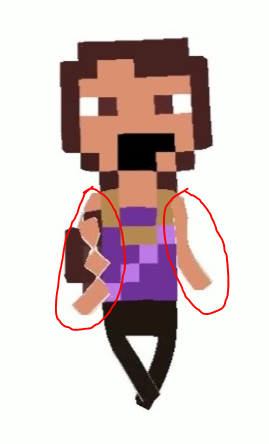
\includegraphics[width=0.3\linewidth]{figs/sketchLab/bracos.PNG}
    \legend{\small Fonte: Elaborada pela autora, utilizando a ferramenta Animated Drawnings.}
\end{figure}


Levando esse fator em consideração, um terceiro sprite é desenhado (Figura \ref{fig:sketchIrma3} para que os braços tenham o mesmo formato durante as animações. Nesse teste, a ferramenta foi capaz de identificar o personagem com muito mais precisão, não sendo necessário fazer nenhuma correção manual na etapa de Destacar personagem. As animações resultantes\footnote{https://drive.google.com/drive/folders/1GklV-37RprR4LGQN-1lyjayqs-gPcpDl?usp=sharing} ainda mantiveram a quebra no pixel perfect, contudo de forma menos acentuada quanto nos casos anteriores. A análise dos resultados também revelou uma nova limitação: a ferramenta considera o cabelo como parte do torso, não compreendendo a diferença de profundidade entre os dois elementos, causando uma sobreposição incorreta do cabelo em relação ao braço. Capturas de tela das animações criadas podem ser consultadas na Figura \ref{fig:sketchIrma3Frame}, e imagens da interação completa podem ser encontradas na Figura \ref{fig:sketch3} no Apêndice \ref{ap.telasIA}.

%Capturas de tela das animações criadas podem ser consultadas na Figura \ref{fig:sketchIrma3Frame}, e imagens da interação completa podem ser encontradas na Figura \ref{fig:sketch3}. Analisando os resultados, foi descoberto que a ferramenta considera o cabelo como parte do torso, não entendendo a diferença de profundidade que ambos possuem, o que pode ser observado na Figura \ref{fig:sketchIrma3Frame2}.

\begin{figure}[htbp]
    \centering
    \caption{\small Frames das animações geradas pelo Animated Drawnings 3}
    \label{fig:sketchIrma3Frame}
    \begin{subfigure}{0.2\linewidth}
        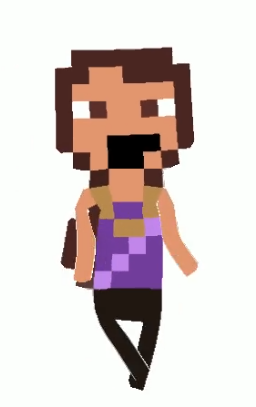
\includegraphics[width=1\linewidth]{figs/sketchLab/bracosIguais.PNG}
        \caption{\small Frame da animação de andar}
        \label{fig:sketchIrma3Frame1}
    \end{subfigure}
    \begin{subfigure}{0.2\linewidth}
        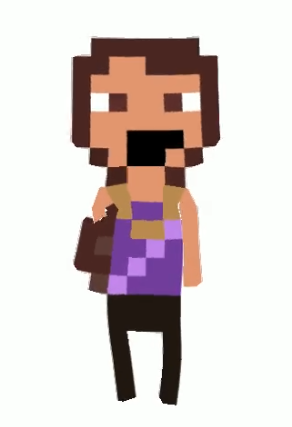
\includegraphics[width=1\linewidth]{figs/sketchLab/cabelo.PNG}
        \caption{\small Frame da animação de acenar}
        \label{fig:sketchIrma3Frame2}
    \end{subfigure}

    \legend{\small Fonte: Elaborada pela autora, utilizando a ferramenta Animated Drawnings.}
\end{figure}

A abordagem da ferramenta, que consiste em identificar um esqueleto no desenho para então aplicar transformações em cada parte do corpo, apresenta benefícios claros. A consistência do personagem é garantida, pois não há geração de novos quadros. A eficiência também é alta, pois um único esqueleto permite a aplicação de múltiplas animações. Além disso, a interface interativa, que permite a correção da IA em etapas, torna a plataforma prática e evita a repetição de prompts comum em outras ferramentas.

Contudo, a abordagem também possui suas limitações. O número de animações disponíveis é restrito e não customizável. A segmentação de partes do corpo é simplificada, o que pode levar a erros de interpretação, como o ocorrido com o cabelo. Por fim, a ferramenta não é capaz de gerar mudanças de ângulo complexas, limitando-se a espelhar a imagem.

%% mudar se acabar usando a animação feita ou não

Após todos esses testes, a ferramenta é considerada funcionalmente satisfatória para criar animações de personagens 2D, embora seja inadequada para o estilo visual do projeto. 

%após foi selecionado as articulações, o algoritmo preve qual a pose e usa as articulações para formar um  rigged character, com partes específicas do corpo, que são renderizadas em ordens diferentes para dar a ilusão de uma parte estar atrás ou a frente

